\documentclass[fleqn]{article}

\usepackage{mydefs}
\usepackage{notes}
\usepackage{url}
\usepackage{graphicx}
\usepackage{textcomp}
\usepackage{hyperref}

\begin{document}
\lecture{Machine Learning \& Discovery}{HW1: Decision trees and KNN}{ECS 271, Fall 2025}

\section{ Math Practice (NOT GRADED)}
% The following are true/false questions.  You don't need to answer the
% questions.  Just tell us which ones you can't answer confidently in
% less than one minute.  (You won't be graded on this.)  If you can't
% answer at least $8$, you should probably spend some extra time outside
% of class beefing up on elementary math. I would strongly suggest going through this math tutorial by Hal Daume:
% https://web.cs.ucdavis.edu/\%7Ehpirsiav/courses/MLf23/math4ml.pdf
\begin{enumerate}
\setlength{\itemsep}{1.2\baselineskip}
\item $\ddx \log x = - \frac 1 x$
\item $p(a, b | c) = \frac{p(a | c)p(b | c)}{p(c)}$
\item $p(a \| b) = p(a,b) / p(b)$
\item $\log x + \log y = \log (xy)$
\item $p(x \| y,z) = p(x \| y) p(x \| z)$
\item $\int_{-\infty}^{\infty} \ud x \exp[-(\pi/2) x^2] = \sqrt{2}$
\item $\log [ab^c] = \log a + (\log b) (\log c)$
\item $\ddx \sigma(x) = \sigma(x)\times(1-\sigma(x))$ where $\sigma(x) = 1/(1+e^{-x})$
\item The distance between the point $(x_1,y_1)$ and line $ax + by + c$ is ${(ax_1 + by_1+c)}/{\sqrt{a^2 + b^2}}$

\item $\ab{\vec u\T\vec v} \geq \norm{\vec u} \times \norm{\vec v}$, where $\ab{\cdot}$ denotes absolute value and $\vec u\T\vec v$ is the dot product of $\vec u$ and $\vec v$
\item $C(n,k) = C(n-1, k-1) + C(n-1, k)$, where $C(n,k)$ is the number of ways of choosing $k$ objects from $n$
\item $\norm{\al \vec u + \vec v}^2 = \al^2 \norm{\vec u}^2 + \norm{\vec v}^2$, where $\norm{\cdot}$ denotes Euclidean norm, $\al$ is a scalar and $\vec u$ and $\vec v$ are vectors

\end{enumerate}
\section{Continuous Variable vs Discrete Variables}
All the attributes we observed in the class so far for decision tree are binary like "Is it Morning?". Now lets assume that our attributes are numerical.
% In class, we looked at an example where all the attributes were binary (i.e., yes/no valued). Consider an example where instead of the attribute ``Morning?", we had an attribute ``Time" which specifies when the class begins.
\begin{enumerate}
    \item  Let's say we want to consider the \textbf{Time} on which the class begins. One can argue that we can pick a threshold $\tau$ and use (Time $< \tau$)? as a criteria to split the data in two and make a binary tree. Explain how you might pick the optimal value of $\tau$.

      For a continuous attribute like \textbf{Time}, we can consider all the unique values of \textbf{Time} in our training data.
      For example, the training data may have times 9:00, 11:00, 12:00, and 16:00.
      Unlike the yes/no case where we only have a single potential boundary, we now can consider splitting at any time between the times in our training data. 
      A simple way to do this would be to take the midpoint between each pair of consecutive unique values in the training data.
      In our example, this would mean our candidates for $\tau$ would be 10:00 (between 9:00 and 11:00), 11:30 (between 11:00 and 12:00), or 14:00 (between 12:00 and 16:00).
      We can then evaluate each candidate $\tau$ as we did for binary attributes, but this time across all candidate thresholds of a continuous attribute.
      In other words, we assign a score like misclassification error (what we did in lecture), information gain, or Gini impurity to each candidate $\tau$ and pick the one that optimizes our chosen score.


    \item In the decision tree learning algorithm discussed in class, once a binary attribute is used, the subtrees do not need to consider it anymore. Explain why in using continuous attributes this may not be the case.
    % \item Now, lets look at a simple problem. Suppose you know that the probability of a dining hall being crowded is made of three normal distribution, with means of 8 (for breakfast), 13 (for lunch), and 18 (for dinner) all have $\sigma = 1$. Given that you're so busy and want to go to the dining hall when there are not so many people there, you have a few meetings, and also you don't want to go to campus on a rainy day, can you build a decision tree to tell you when should you go to a dining hall?
\end{enumerate}

% \begin{solution}
%   $\tau = \argmin (f(x))$
% \end{solution}

% \begin{solution}
% Think of a clever answer
% \end{solution}


\section{To Memorize or Not to Memorize:}
% Why memorizing the training data and doing table lookups is a bad strategy for learning? How do we prevent that in decision trees?
Why using the training data as a dictionary or lookup table and referring to it is a bad strategy for learning? What is it called? How do we prevent it?

% \begin{solution}
% "if you tell the truth, you don't have to remember anything" - Mark twain
% \end{solution}

\section{Visualize} What does the decision boundary of 1-nearest neighbor classifier for 2 classes (one positive, one negative) look like when the features are 1-D? How about 2-D and 3-D? Can you give a general form?
% \begin{solution}
% \end{solution}

\section{kNN and data manipulation}

Does the accuracy of a kNN classifier using the Euclidean distance change if you:(a) translate the data (b) scale the data (i.e., multiply all the points by a constant), or (c) rotate the data? Explain. Answer the same for a kNN classifier using Manhattan distance\footnote{\url{http://en.wikipedia.org/wiki/Taxicab_geometry}} and Cosine Distance\footnote{\url{https://en.wikipedia.org/wiki/Cosine_similarity}}. Make sure you provide mathematical proofs or at least some intuition that why your claim is correct.
% \begin{solution}
% \end{solution}

\section{Coding}

Implement kNN in Python for handwritten digit classification and submit all codes and plots:

Download MNIST digit dataset (60,000 training and 10,000 testing data points) and the starter code from the course page. Each row in the matrix represents a handwritten digit image. The starter code shows how to visualize an example data point. The task is to predict the class (0 to 9) for a given test image, so it is a 10-way classification problem.

\begin{figure}[h]
\centering
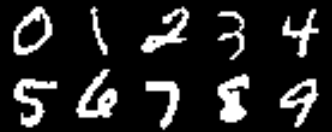
\includegraphics[width=.4\linewidth]{mnist-dataset.png}
\end{figure}


\begin{enumerate}


\item Write a Python function that implements kNN for this task and reports the accuracy for each class (10 numbers) as well as the average accuracy (one number).

{\em [acc acc\_av] = kNN(images\_train, labels\_train, images\_test, labels\_test, k)}

where {\em acc} is a vector of length 10 and {\em acc\_av} is a scalar. Look at a few correct and wrong predictions to see if it makes sense. To speed it up, in all experiments, you may use only the first 1000 testing images.

\item For $k=1$, change the number of training data points (30 to 10,000) to see the change in performance. Plot the average accuracy for 10 different dataset sizes. In the plot, x-axis is for the number of training data and y-axis is for the accuracy.

\item Show the effect of $k$ on the accuracy. Make a plot similar to the above one with multiple colored curves on the top of each other (each for a particular $k$ in [1 3 5 10].)

\item Choose the best $k$. First choose 2,000 training data randomly (to speed up the experiment). Then, split the training data randomly to two halves (the first for training and the second for cross-validation to choose the best $k$). Please plot the average accuracy wrt $k$ on the validation set. You may search for $k$ in this list: [1 3 5 10]. Finally, report the accuracy for the best $k$ on the testing data.

\end{enumerate}
\end{document}
